\documentclass[11pt]{article}
\usepackage{fancyhdr}
\usepackage{graphicx}
\usepackage{amssymb,amsmath}
\usepackage{psfrag}
\usepackage{color}
\usepackage[colorlinks]{hyperref}
\usepackage[footnotesize,hang,bf]{caption}
\usepackage{subeqnarray}
% \usepackage{amsthm}
 \usepackage{enumitem}
 \graphicspath{{Figures/}}
 \usepackage{multicol}
 \usepackage{ marvosym }
 \usepackage{wasysym}
 \usepackage{tikz}
 \usetikzlibrary{patterns}

 \newcommand{\ds}{\displaystyle}
 \DeclareMathOperator{\sech}{sech}

%%%%%%%%%%%%%%%%%%%%%%%%%%%%%%%%%%%%%%%%%%%%%%%%%%%%%%%%%%%%%%%%%%%%%%%%%%%%%%%%%%

\def\hwnum{2}
\def\term{Spring 2017}

\textwidth = 6.0 in
\textheight = 8.5 in
\oddsidemargin = 0.0 in
\evensidemargin = 0.0 in
\topmargin = -0.5 in
\headheight = 0.6 in
\headsep = 0.2 in
\renewcommand{\baselinestretch}{1}


\pagestyle{fancy}
\rhead{ME 257/357\\ \term \\Problem Set \#\hwnum}
\lhead{}
\renewcommand{\headrulewidth}{0pt}

\begin{document}

\begin{center}
{\Large\bf ME 257/357 Gas Turbine Design: Problem Set \#\hwnum\\
       Due: Monday, 5/1/2017 (before lecture)}
\end{center}

%=======================================================================================================
Before solving this problem set, outline the approach you want to follow. Provide all solution steps, and clearly mark your solution. Start with the general formulation, and simplify all expressions as much as possible. Plug in all numbers only at the end. Make and state necessary assumptions that you
think are required for solving the problem. You are encouraged to discuss the approach you want to follow on a conceptual level in groups; however, you have to submit your own write-up, plots, and non-trivial source code.
\\
\hrule
%=======================================================================================================
\section{Equilibrium Combustion}
%=======================================================================================================
In this problem we consider the combustion of dodecane ($\mathrm{C_{12}H_{26}}$, close to kerosene or Jet-A, JP-8, etc. jet fuels) with air at 1 atm pressure.  The temperature of both reactants is 500 K.  The primary objective of this problem is to give you experience in writing your own equilibrium solver and expose you to NASA polynomial tables for thermochemical species.
%=======================================================================================================
\subsection{Stoichiometry}
%=======================================================================================================
\begin{enumerate}[label=(\alph*)]
	\item
    	Write equations for stoichiometric, fuel-lean, and fuel-rich dodecane/air combustion.  Assume that only the stable products $\mathrm{CO_2}$ and $\mathrm{H_2O}$ are formed and that the excess of reactants is not dissociated on the product side.  Use atomic balance and express all stoichiometric coefficients as functions of $\phi$.
    \item
    	Evaluate the species product mass fractions of $\mathrm{CO_2}$ and $\mathrm{H_2O}$ as functions of $\phi$, and plot your results for $0 \le \phi \le 2$.
\end{enumerate}
%=======================================================================================================
\subsection{Adiabatic Flame Temperature}
%=======================================================================================================
We will now proceed by extending our code to compute the adiabatic flame temperature.  We will first consider a calorically perfect gas model for the combustion, and we will then consider the results from an equilibrium solver.

\begin{enumerate}[label=(\alph*)]
	\item
    	Use Table~\ref{TAB_HEATS}, and derive an expression for the heat of combustion as a function of $\phi$ for general reactant temperature and pressure (since combustion in a gas turbine takes place at high pressure and temperature).  Is this reaction exothermic or endothermic?
        
        \begin{table}[!htb!]
        	\centering
        	\begin{tabular}{|p{0.3\textwidth}|p{0.25\textwidth}|p{0.25\textwidth}|}\hline
        Species & Formation Enthalpy, $\Delta H_\mathrm{ref}^\circ$(298 K) [J/kg]& Constant-Pressure Specific Heat Ratio, $c_p$ [J/kg.K] \\ \hline
        Dodecane: C$_{12}$H$_{26}$ (g) & -1.71$\times 10^6$ & 3.372$\times 10^3$ \\
        Water Vapor: H$_{2}$O (g) & -13.4$\times 10^6$ &  2.38$\times 10^3$\\
        Carbon Dioxide: CO$_{2}$ (g) & -8.94$\times 10^6$  & 1.22$\times 10^3$\\
        Oxygen: O$_{2}$ (g) & 0 (Reference Species) & 1.09$\times 10^3$\\
        Nitrogen: N$_{2}$ (g) & 0 (Reference Species) & 1.18$\times 10^3$\\
        \hline
        \end{tabular}
          \caption{\label{TAB_HEATS}Table of formation enthalpies and the specific heat ratios for the species of interest.}
          \end{table}
    \item
    	Compute the adiabatic flame temperature for $0 \le \phi \le 2$.  Recall that combustion occurs at nearly constant pressure; assume that the specific heat is constant and use the expression $\mathrm{d} h=c_p\mathrm{d}T$.
    \item
    	Use \href{http://navier.engr.colostate.edu/~dandy/code/code-4/}{STANJAN}, \href{https://cearun.grc.nasa.gov/}{CEA}, or \href{http://www.cantera.org/docs/sphinx/html/index.html}{cantera} (recommended) to compute the adiabatic flame temperature for constant-pressure/enthalpy conditions $0 \le \phi \le 2$.
    \item
    	Compare your results for the constant specific model and the equilibrium solver on the same plot. What differences in the two models may be causing discrepancies and why? 
\end{enumerate}	

%=======================================================================================================
\section{Gas Turbine Combustor Design}
%=======================================================================================================
For this problem, we will be exploring the design of a Rich Burn, Quick-Mix, Lean Burn (RQL) combustor. A schematic of this combustor is shown in Fig.~\ref{FIG_RQL}. In an RQL combustor the fuel-air mixture is initially burned rich ($\phi>1$) to limit NO$_\mathrm{x}$ formation through oxygen depletion and the relatively low combustion temperature. However, additional air needs to be injected to minimize other pollutants resultant from the rich burn (e.g., CO). Hence, a secondary mixing process is undergone by injecting air subsequent to the rich zone to yield a lean condition downstream. Similar to rich combustion, the nitric oxide (NO) formation is reduced for lean conditions as shown in the figure.

\begin{figure}[!ht!]
	\begin{center}
		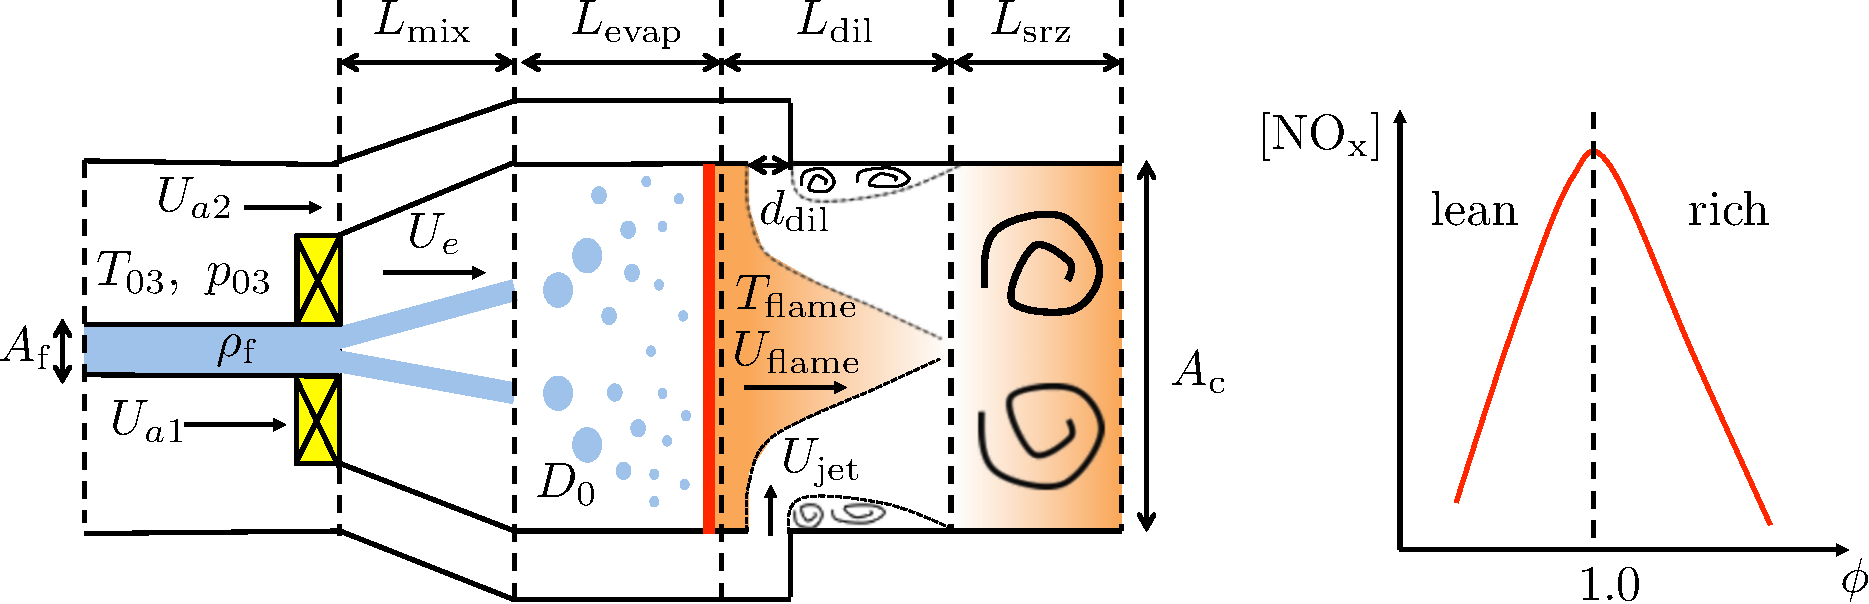
\includegraphics[width=0.9\textwidth]{RQLCombustor.png}
		\caption{\label{FIG_RQL} Schematic of a RQL combustor and the effect of equivalence ratio, $\phi$, on combustion.}
	\end{center}
\end{figure}
%=======================================================================================================
\subsection{Combustor Inlet Conditions}
%=======================================================================================================
In this problem we wish to uncover the inlet conditions of the combustor with respect to the operational conditions. For simplicity, consider this combustor to be a part of an ideal turbojet system.
\begin{enumerate}
	\item
    	Given $T_{04}/T_0,\ T_{03}/T_{02},\ T_{00}/T_{0}$, and LHV$/(c_pT_0)$, determine the fuel-air ratio of the combustor.
    \item
    	For n-dodecane, what is the overall stoichiometry of the combustor in terms of the fuel-air ratio? 
    \item
    	Assuming the Mach number in the combustor is much less than unity, what is the static temperature and pressure to the inlet of the combustor?
\end{enumerate}
%=======================================================================================================
\subsection{Combustor Diameter}
%=======================================================================================================
For this homework, we will considered a canned combustor geometry. Canned combustors are discrete units with their own casing, fuel injection, liner, and igniter. Other designs include annular and cannular combustors. We will assume for this problem that the combustor geometry is strictly cylindrical and axisymmetric. 

\begin{figure}[!ht!]
	\begin{center}
		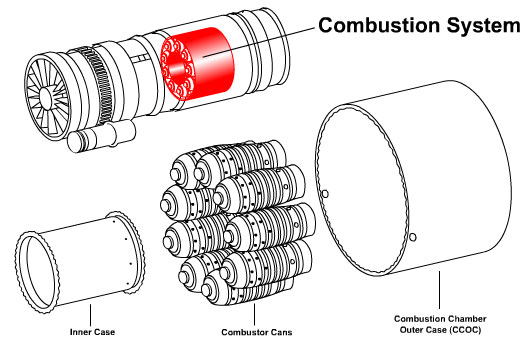
\includegraphics[width=0.9\textwidth]{cannedCombustor.jpg}
		\caption{\label{FIG_CC} Schematic of a canned combustor system}
	\end{center}
\end{figure}

\begin{enumerate}[label=(\alph*)]
	\item
    	Consider a gas-turbine engine with a circular array of canned combustors as shown in the figure. The outer case has specified outer radius, $R_\mathrm{o}$, and inner case radius, $R_\mathrm{i}$. Using this, what is the maximum number of canned combustors that may fit in the annular section? What is the diameter, $D_\mathrm{c}$ of each combustor?
\end{enumerate}
%=======================================================================================================
\subsection{Combustor Length}
%=======================================================================================================
In this problem, we are interested in developing a model that will give the minimum length of the RQL combustor. We will assume that the RQL combustor follows the zonal model shown in Fig.(To be included). The combustor is shown to be broken up by physical processes into four zones: atomization and evaporation, flame, mixing, and a perfectly-stirred reactor. In reality, there is significant interplay between these regions and the processes can be quite complex, but the goal here is to develop a low-order model, which contains the essential physics of an RQL combustor. 
\begin{enumerate}[label=(\alph*)]
	\item
    	Assume that each physical process has a representative timescale, $\tau$, and velocity, $U$. Propose a relation, which gives the length of the combustor in terms of the timescale and velocity for each region.
    \item \textit{Atomization and Evaporation}\\
    	In the atomization and evaporation section of the combustor, the fuel is injected as a liquid with a coaxial air flow. Instabilities due to the air-liquid interface cause the liquid jet to break-up and atomize. Subsequently, the atomized droplets will evaporate and mix with the air forming a rich combustible mixture. We will assume that the atomization process is relatively quick compared to the evaporation of the droplets.
        \begin{enumerate}[label=(\roman*)]
        	\item
            	What is the characteristic velocity of the atomization and evaporation section, $U_\mathrm{evap}$, in terms of the ratio of rerouted air to inlet air, $\beta_c=\dot{m}_{a2}/\dot{m}_{a1}$; the air mass flow rate, $\dot m_\mathrm{a}$; the fuel-air ratio, $f$; and the air and fuel densities, $\rho_\mathrm{a}$ and $\rho_\mathrm{f}$, respectively? Assume that the process is approximately isobaric. 
            \item 
            	Under certain assumptions and using conservation of energy in spherical coordinates, the evaporation rate, $\dot m _\mathrm{f}$, of an isolated liquid droplet can be found to be
                \begin{equation}
                	\label{EQ_DROPLET}
                	\begin{aligned}
                    	\dot{m}_\mathrm{evap}=2\pi D \frac{\lambda_\mathrm{g}\log(1+\mathcal{B})}{c_{p\mathrm{g}}}
                    \end{aligned}
                \end{equation}
                where $D$ is the diameter of the droplet, and $\mathcal{B}$ is the Spalding number. Using Eq.~\ref{EQ_DROPLET}, derive the evaporation time of the droplet in terms of the initial diameter $D_0$ and an evaporation constant $\beta=8\lambda_\mathrm{g}\log(1+\mathcal{B})/(\rho_\mathrm{f}c_{p\mathrm{g}})$.
        	\item
            	(BONUS: 2 pts)The Rosin-Rammler expression is commonly used to describe the size distribution of droplet diameters and is given by 
                \begin{equation}
                	\label{EQ_RR}
                	\begin{aligned}
                    	f(D_0;D_\sigma,\alpha)=1-\exp\left[\left(\frac{D_0}{D_\sigma}\right)^\alpha\right]
                    \end{aligned}
                \end{equation}
                where $f$ is the total fraction of fuel contained in droplets of diameter less than $D_0$, and $\alpha$ and $D_\sigma$ are parameters of the distribution. Using Eq.~\ref{EQ_RR} and your result from ii, derive an expression for the mean evaporation time for a droplet in the fuel spray. Assume $\alpha=2$.
        	\item
            	Using your results from i and iii, what is the characteristic length of the atomization and evaporation section of the combustor in terms of $U_\mathrm{evap}$ and the mean evaporation time $\tau_\mathrm{evap}$? 
        \end{enumerate}
    \item \textit{Flame}\\
    	Subsequent to the atomization and evaporation section of the combustor, a turbulent flame combusts the rich fuel-air mixture. In this assignment, we will make the coarse assumption that the flame is completely premixed for simplicity.  
        \begin{enumerate}[label=(\roman*)]
        	\item
            	For a laminar, premixed, and adiabatic free-flame, the flame speed, $S_\mathrm{L}$, under a unity Lewis number assumption can be determined to be
                \begin{equation}
                	\label{EQ_SL}
                	\begin{aligned}
                    	S_\mathrm{L}=\left[-2\alpha(1+f)\frac{\langle\dot m_\mathrm{f}^{\prime \prime \prime}\rangle}{\rho_\mathrm{u}}\right]^{\frac{1}{2}}
                    \end{aligned}
                \end{equation}
                where $\alpha$ is the heat diffusivity, $\langle\dot m_\mathrm{f}^{\prime \prime \prime}\rangle$ is the mean fuel consumption rate across the flame, and $\rho_\mathrm{u}$ is the density of the unburned reactants. Given that $\alpha\propto 1/p$ and $\langle\dot m_\mathrm{f}^{\prime \prime \prime}\rangle\propto p^n$, where $n$ is the overall reaction order, how does the laminar flame speed scale with pressure? Assume $n=1$.
        	\item
            	Under certain assumptions about the topology of turbulent flame, the turbulent flame speed is estimated by
                \begin{equation}
                	\label{EQ_ST}
                	\begin{aligned}
                    	S_\mathrm{T}=S_\mathrm{L}\left[1+\mathcal{I}B\frac{U_\perp}{S_\mathrm{L}}\right]^{\frac{1}{2}}
                    \end{aligned}
                \end{equation}
        	where $\mathcal{I}= u^\prime_\mathrm{RMS}/U_\perp$ is the turbulence intensity, $B$ is a constant of order unity, and $U_\perp$ is the speed normal to the flame brush. Assuming that the flame adjusts to the mean flow velocity in a ``V" configuration that extends from the center of the combustor to the wall, determine the length of the flame in terms of $S_\mathrm{L}$, $\mathcal{I}$, and the characteristic velocity $U_\mathrm{evap}$. Assume that the flame brush thickness is negligible, and that $B=1$. 
            \item
            	Plot $S_\mathrm{L}/U_\mathrm{evap}$ vs $L_\mathrm{flame}/D_\mathrm{c}$ for $\mathcal{I}\in\{0.005, 0.05, 0.5\}$. What effect does turbulence have on the compactness of the flame? What about pressure?
            \item 
            	What is the fluid speed subsequent to the flame, $U_\mathrm{flame}$, in terms of $U_\mathrm{evap}$ and the ratio of adiabatic flame temperature to the unburned reactant temperature, $T_\mathrm{ad}/T_\mathrm{3}$?
            \item
                  Taking the turbulent flame velocity to be the characteristic speed of this portion of the combustor, determine the characteristic timescale of the flame.
            \end{enumerate}
	\item \textit{Mixing}
		
        The mixing section consists of dilution holes injecting air bypassed from the core flow in a jet-in-crossflow configuration. The holes are arranged azimuthally around the combustor.
         \begin{enumerate}[label=(\roman*)]
         	\item
            	Find a relation for the jet velocity $U_{\mathrm{jet}}$ of each hole in terms of the number of holes, $n_\mathrm{hole}$, the diameter of each hole, $d_\mathrm{hole}$, $\rho_\mathrm{a}$, $\dot m_\mathrm{a}$, and $\beta_\mathrm{c}$.
            \item
            	In the far-field, a jet-in-crossflow displays the self-similar scaling of 
                \begin{equation}
                	\begin{aligned}
                    	c\sim \left(\frac{L}{rd_\mathrm{hole}}\right)^{-\frac{2}{3}}
                    \end{aligned}
                \end{equation}
                where $c$ is the concentration, $L$ is the distance after injection, and the momentum ratio is given in therms of the jet and crossflow momentums as
                \begin{equation}
                	\label{EQ_JIC}
                	\begin{aligned}
                	r=\sqrt{\frac{\rho_\mathrm{jet}U_\mathrm{jet}^2}{\rho_\mathrm{cf}U_\mathrm{cf}^2}}
                    \end{aligned}
                \end{equation}
         
           What is the final concentration $c_\mathrm{f}$ in terms of $\dot m_\mathrm{a}$, $f$, and $\beta_\mathrm{c}$?
           \item
              Approximate the length of mixing region using the scaling relationship presented in Eq.~\ref{EQ_JIC}.
           \item
           		What is bulk velocity of the fluid subsequent to the mixing process, $U_\mathrm{mix}$?
         \end{enumerate}
    \item \textit{Perfectly Stirred Reactor}
    
    	The zone subsequent to the jet and cross flow mixing process is assumed to be highly turbulent and without prominent flame structure. In this section of the flow, it is assumed that the relevant timescale of the flow is given by the ignition delay:
        \begin{equation}
          \label{EQ_IGN}
          \begin{aligned}
            \tau_\mathrm{ign}=\frac{A}{\phi p^n}\exp\left(\frac{E_\mathrm{a}}{RT}\right)
          \end{aligned}
        \end{equation}
        \begin{enumerate}[label=(\roman*)]
        \item
        	Determine $\phi$ in the perfectly stirred reactor (PSR) section of the combustor.
        \item
        	Using Eq.~\ref{EQ_IGN}, find the length of the PSR. 
        \end{enumerate}
	\item
    	Using the values in Table~\ref{}, compute the total length of the combustor.
\end{enumerate}
%=======================================================================================================
\subsection{Emissions and Pollutant Formation}
%=======================================================================================================
*present empirical relations in for NO$_\mathrm{x}$; ask student to compute NO$_\mathrm{x}$ for the a non RQL combustor.
%=======================================================================================================
\bibliographystyle{unsrt}
\bibliography{combustion,shocktube}
%=======================================================================================================
\end{document}